\documentclass[12pt, a4paper, oneside, UTF8]{ctexart}
\usepackage{amsmath, amsthm, amssymb, bm, color, framed, graphicx, hyperref, mathrsfs}
\usepackage{geometry}
\geometry{left = 2.5 cm, right = 2.5 cm, top = 2.5 cm, bottom = 2.5 cm}

\title{\textbf{作业2}\\{\small (数值算法与案例分析)}}
\author{李维杰}
\date{\today}
\linespread{1.5}
\definecolor{shadecolor}{RGB}{241, 241, 255}
\newcounter{problemname}
\newenvironment{problem}{\begin{shaded}\stepcounter{problemname}\par\noindent\textbf{题目\arabic{problemname}. }}{\end{shaded}\par}
\newenvironment{solution}{\par\noindent\textbf{解答. }}{\par}
\newenvironment{note}{\par\noindent\textbf{注记. }}{\par}

\begin{document}

\maketitle

\begin{problem}
    针对复矩阵的高斯消元/LU分解,其执行过程中加减/乘法运算的操作次数是否相等?
\end{problem}

\begin{solution}
    设对于同一大小的实矩阵进行高斯消元/LU分解时,执行过程中加减和乘法运算的次数分别为$p_1,p_2$.另设$z_1=a_1+b_1{i},z_2=a_2+b_2{i}$,则复数加减操作为
    \begin{align*}
        {z_1}\pm{z_2}=({a_1}\pm{a_2})+({b_1}\pm{b_2}){i}.
    \end{align*}
    即复数加减操作的运算次数$q_1=2p_1$.\\
    复数的乘法操作为
    \begin{align*}
        {z_1}{z_2}=({a_1}{a_2}-{b_1}{b_2})+({a_1}{b_2}+{a_2}{b_1}){i}.
    \end{align*}
    即复数乘法操作的运算次数$q_2=2{p_1}+4{p_2}$.\\
    又已知$p_1=p_2$,故$q_2=3q_1$,即复矩阵在高斯消元/LU分解的过程中,执行加减/乘法运算的操作次数不相等.
\end{solution}
\newpage
\begin{problem}
    用两种算法求对称正定阵$A$的Cholesky分解.(即求下三角阵$L$,满足$A={L}{L^T}$)
\end{problem}

\begin{solution}
    \par \textbf{算法1}\\
        设
        \begin{align*}
            L=
            \left[
            	\begin{array}{cccc}	
            	l_{11}\\	
            	l_{21} & l_{22} \\	 
                \vdots & \vdots & \ddots \\
           	  	l_{n1} & l_{n2} & \cdots & l_{nn}
            	\end{array}
            \right].
        \end{align*}
        则由$A=LL^T$,得
        \begin{align}
            a_{ij}=\sum\limits_{k=1}^{j}{l_{ik}}{l_{jk}},&&{1}\leq{j}\leq{i}\leq{n}.
        \end{align}
        对于第$1$列,由式(1)在$j=1$时的特例$a_{i1}=l_{i1}l_{11}$,即得
        \begin{align*}
            l_{i1}=\frac{a_{i1}}{l_{11}}.
        \end{align*}
        特别地,有$$a_{11}=(l_{11})^2\Rightarrow{l_{11}}=\sqrt{a_{11}},$$
        从而可以计算得$L$阵的第$1$列元素.\\
        对于第$j$列,由式(1)可得
        \begin{align*}
            l_{ij}=\frac{a_{ij}-\sum\limits_{k=1}^{j-1}l_{ik}l_{jk}}{l_{jj}}.
        \end{align*}
        特别地,有$$a_{jj}=\sum\limits_{k=1}^{j}{(l_{jk})^2}\Rightarrow{l_{jj}=\sqrt{a_{jj}-\sum\limits_{k=1}^{j-1}(l_{jk})^2}},$$
        从而可以递推计算得$L$阵所有元素.
    \par \textbf{算法2}\\
        设$L_0$为单位下三角阵,设$D$是对角元均为正数的对角阵,令$A={L_0}D{L_0}^{T}$,得
        \begin{align}
            a_{ij}=\sum_{k=1}^{j-1}{l_{ik}d_{k}l_{jk}}+l_{ij}d_{j},&&{1}\leq{j}\leq{i}\leq{n}.
        \end{align}
        对于第$1$列,由式(2)在$j=1$时的特例$a_{i1}=l_{i1}d_{1}$,即得
        \begin{align*}
            l_{i1}=\frac{a_{i1}}{d_{1}}.
        \end{align*}
        对于第$j$列,由(2)式可得
        \begin{align*}
            l_{ij}=\frac{a_{ij}-\sum\limits_{k=1}^{j-1}{l_{ik}d_{k}l_{jk}}}{d_{j}}.
        \end{align*}
        特别地,当$i=j$时,有$l_{ij}=1$,则
        \begin{align*}
            d_{j}=a_{jj}-\sum_{k=1}^{j-1}{l_{jk}d_{k}l_{jk}}.
        \end{align*}
        从而通过递推计算得$L_0$阵和$D$阵的所有元素,进而得到
        \begin{align*}
            L=
            \left[
            	\begin{array}{cccc}	
            	d_{1}\\	
            	l_{21} & d_{2} \\	 
                \vdots & \vdots & \ddots \\
           	  	l_{n1} & l_{n2} & \cdots & d_{n}
            	\end{array}
            \right].
        \end{align*}
\end{solution}

\begin{problem}
    证明:严格对角占优的矩阵$A$在高斯消元过程中得到的子矩阵依然严格对角占优.
\end{problem}

\begin{solution}
    设
    \begin{align*}
        P=
        \left[
            \begin{array}{ccccc}	
            1\\	
            -\frac{a_{21}}{a_{11}} & 1 \\
            -\frac{a_{31}}{a_{11}} & 0 & 1 \\ 
            \vdots & & & \ddots \\
           	-\frac{a_{n1}}{a_{11}} & 0 & 0 & \cdots & 1
            \end{array}
        \right].
    \end{align*}
    设一步高斯消元后得到的矩阵为$B=PA$,则
    \begin{align*}
        b_{ij}=a_{ij}-\frac{a_{i1}a_{1j}}{a_{11}}.
    \end{align*}
    于是
    \begin{align*}
        \sum\limits_{\substack{{2}\leq{j}\leq{n}\\{j}\neq{i}}}{\left\lvert {b_{ij}}\right\rvert }&=\sum\limits_{\substack{{2}\leq{j}\leq{n}\\{j}\neq{i}}}{\left\lvert {a_{ij}-\frac{a_{i1}a_{1j}}{a_{11}}}\right\rvert }\\
        &\leq\sum\limits_{\substack{{2}\leq{j}\leq{n}\\{j}\neq{i}}}{\left\lvert {a_{ij}}\right\rvert }+\sum\limits_{\substack{{2}\leq{j}\leq{n}\\{j}\neq{i}}}{\left\lvert {\frac{a_{i1}a_{1j}}{a_{11}}}\right\rvert }\\
        &=\sum\limits_{\substack{{2}\leq{j}\leq{n}\\{j}\neq{i}}}{\left\lvert {a_{ij}}\right\rvert }+{\left\lvert {\frac{a_{i1}}{a_{11}}}\right\rvert }\sum\limits_{\substack{{2}\leq{j}\leq{n}\\{j}\neq{i}}}{\left\lvert {a_{1j}}\right\rvert }\\
        &=\sum\limits_{\substack{{1}\leq{j}\leq{n}\\{j}\neq{i}}}{\left\lvert {a_{ij}}\right\rvert }-{\left\lvert {a_{i1}}\right\rvert}+{\left\lvert {\frac{a_{i1}}{a_{11}}}\right\rvert }\sum\limits_{{2}\leq{j}\leq{n}}{\left\lvert {a_{1j}}\right\rvert }-{\left\lvert {\frac{a_{i1}a_{1i}}{a_{11}}}\right\rvert }\\
        &<{\left\lvert{a_{ii}}\right\rvert}-{\left\lvert{a_{i1}}\right\rvert}+{\left\lvert{a_{i1}}\right\rvert}-{\left\lvert {\frac{a_{i1}a_{1i}}{a_{11}}}\right\rvert }\\
        &<{\left\lvert{a_{ii}-\frac{a_{i1}a_{1i}}{a_{11}}}\right\rvert}\\
        &={\left\lvert {b_{ii}}\right\rvert}.
    \end{align*}
    从而矩阵$B$严格对角占优.
\end{solution}

\begin{problem}
    比较全主元三角分解和列主元三角分解的效率.
\end{problem}

\begin{solution}
    全主元三角分解(红线)和列主元三角分解(蓝线)在不同大小的系数矩阵下的运行效率关系图如下
    \begin{figure}[htbp]
        \centering
        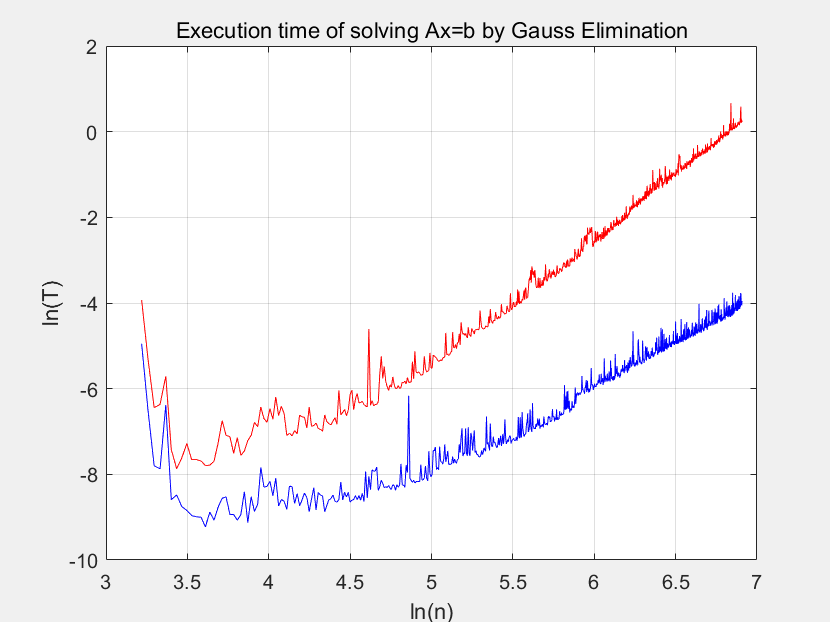
\includegraphics[scale=0.4]{Problem4.png}
    \end{figure}
\end{solution}

\begin{problem}
    证明:存在误差矩阵$E$,使得$(A+E)x=fl(Ax)$.并确定$E$中元素的上界.
\end{problem}

\begin{solution}
    设$b=Ax=(b_1,b_2,...,b_m)^T$,则
    \begin{align*}
        b_i=\sum_{j=1}^{n}{a_{ij}x_{j}}.
    \end{align*}
    设
    \begin{align*}
        S_{ik}=fl(\sum\limits_{j=1}^{k}{a_{ij}x_{j}}),
    \end{align*}
    则
    \begin{align*}
        S_{i1}&=a_{i1}x_{1}(1+\gamma_{i1}),\left\lvert{\gamma_{i1}}\right\rvert\leq\textbf{u}.\\
        S_{ik}&=fl[S_{i(k-1)}+fl(a_{ik}x_{k})]\\&=[S_{i(k-1)}+a_{ik}x_{k}(1+\gamma_{ik})](1+\delta_{ik}),\left\lvert{\gamma_{ik}}\right\rvert,\left\lvert{\delta_{ik}}\right\rvert\leq\textbf{u}.
    \end{align*}
    故
    \begin{align*}
        fl(b_i)=S_{in}=\sum_{j=1}^{n}{a_{ij}x_{j}(1+\gamma_{ij})\prod_{k=j}^{n}{1+\delta_{ik}}}.
    \end{align*}
    令$1+\varepsilon_{ij}=(1+\gamma_{ij})\prod\limits_{k=j}^{n}{(1+\delta_{ik})}$,则
    \begin{align*}
        fl(b_i)=\sum_{j=1}^{n}{(1+\varepsilon_{ij})a_{ij}x_{j}}=\sum_{j=1}^{n}{(a_{ij}+\varepsilon_{ij}a_{ij})x_{j}}.
    \end{align*}
    其中
    \begin{align*}
        \varepsilon_{ij}&=(1+\gamma_{ij})\prod\limits_{k=j}^{n}{(1+\delta_{ik})}-1\\
        &\leq(1+\textbf{u})(1+\textbf{u})^{n-j+1}-1\\
        &\leq(1+\textbf{u})e^{(n-j+1)\textbf{u}}-1\\
        &\leq(1+\textbf{u})[1+1.01(n-j+1)\textbf{u}]-1\\
        &=1.01(n-j+2)\textbf{u}+o(\textbf{u}^2).
    \end{align*}
    则对于误差矩阵$E=(e_{ij}),i,j=1,2,...,n$,有
    \begin{align*}
        \left\lvert{e_{ij}}\right\rvert=\left\lvert{\varepsilon_{ij}a_{ij}}\right\rvert\leq1.01(n-j+2)\left\lvert{a_{ij}}\right\rvert\textbf{u}.
    \end{align*}
    其中\textbf{u}是机器精度.
\end{solution}

\end{document}